Graph Theory is a branch of Mathematics and Computer Science whose goal is the study of graphs. These ones are objects which allows to schematize situations, processes in order to analize them in quantitative and algorithmic terms. They are also object of study mainly in Computer Science thanks to the development of specific algorithms. In graph theory there are a lot of problems: one of the most famous is about the Perfect Matching. Before we introduce it, we are going to recall some useful definition, notions and results.

% 1.1
\section{Some Generalities about Graphs}
\begin{definition}
We define $graph$ a ordered pair $G$ $=$ $(V,E)$ comprising a set V of vertices (or nodes) together with a set E of edges (or arcs) which are 2-element subsets of V.\\
\\
Given a graph G, with |V(G)| we denote the order of G, i.e the number of vertices of G while with |E(G)| we denote the size of G, i.e the number of edges of G\\
\\
A vertex $v \in V$ is incident to an edge $e \in E$ se $v \in e$.\\
Two edges $e_{1}, e_{2} \in E$ are incident (or adjacent) if they are a common vertex.\\
Two vertices $v_{1}, v_{2} \in V$ are adjacent if there exist an edge e $\in E$ such that $e=v_{1}v_{2}$.
\end{definition}

\begin{definition}
Let $G$ $=$ $(V,E)$ e $G'$ $=$ $(V',E')$ be two graphs. If $V'\subseteq V$ and $E'\subseteq E$, then $G'$ is a subgraph of $G$.
Moreover, if $G\ne G$, then we say that $G'$ is a proper subgraph of $G$.
\end{definition}

\begin{definition}
Let $G$ $=$ $(V,E)$ be a graph and let $v \in V$ be a vertex. The degree of a vertex $v$ is defined as
\begin{equation*}
d_{G}(V) := |N_{G}(v)|
\end{equation*}
where $N_{G}(v) := \left \{ w \in V : vw \in E \right \}$ is the neighbour of v. In other words, it is the number of edges incident to the vertex $v \in V$.
Next, we define
\begin{equation*}
\delta(G) := \min\limits_{v \in V} d_{G}(v) \in \mathbb{Z}
\end{equation*}
the minimum degree of G, i.e. the degree of the vertex of less incident edges and
\begin{equation*}
\Delta(G) := \max\limits_{v \in V} d_{G}(v) \in \mathbb{Z}
\end{equation*}
the maximum degree of G, i.e. the degree of the vertex with more incident edges.
Furthermore, we denote the average degree of G as
\begin{equation*}
d(G) := \frac{1}{|V|} \sum_{v \in V} d_{G}(v)
\end{equation*}
Obviously, we have that $\delta(G) \le d(G) \le \Delta(G)$.
\end{definition}

\begin{definition}
A graph $G$ $=$ $(V,E)$ is said to be K-regular if 
\begin{equation*}
d_{G} = k \qquad \forall v \in V
\end{equation*}
In other words, if all vertices have the same degree. As a consequence, we have $\delta = d = \Delta$.
In particular, 3-regular graphs are called also cubic graphs.
\end{definition}

\begin{definition}
A path is a graph $P = (V,E)$ on the form $V = \left \{x_{0}x_{1}, x_{1}x_{2}, \dots, x_{k-1}x_{k} \right \}$ where\\
$x_{0}$ e $x_{k}$ are called ends of P;\\
$x_{2}, \dots, x_{k-1}$ are the inner vertices of P;\\
The number of edges is the length of P;\\ 
With $P_{k}$ we mean a path of lenght $k$.
\end{definition}

\begin{definition}
A graph is said to be complete if every vertex is linked to all remaining vertices . It is denoted with $K_{n}$ (with $n \in N $ the number of vertices)
\end{definition}

\begin{definition}
A graph $G$ $=$ $(V,E)$ is bipartite if its vertex set $V$ can be partitioned into two disjoint subsets $V$ $=$ $V_{1} \cup V_{2}$ such that every edge $e \in E$ has the form $v_{1}v_{2}$, with $v_{1} \in V_{1}$ and $v_{2} \in V_{2}$.
\end{definition}

\begin{definition}
We define a planar graph $G$ a graph such that it can be rapresented  in a plane in order that they do not admite edges who intersect each other.\\
The complete graphs $K_{5}$ e $K_{3,3}$ are non-planar graphs.
\end{definition}
We report some example:

\begin{figure}[htbp]
\begin{minipage}[htbp]{.50\textwidth}
\centering
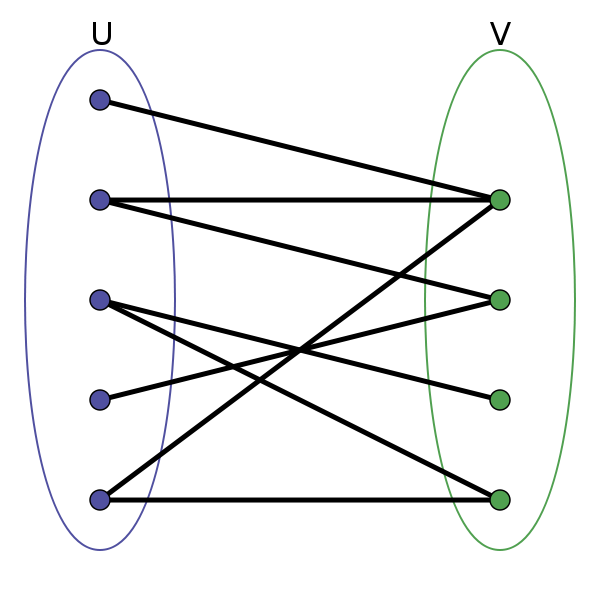
\includegraphics[width=.60\textwidth]{bipartito.png}
\caption{Bipartite graph}
\end{minipage}
\begin{minipage}[htbp]{.50\textwidth}
\centering
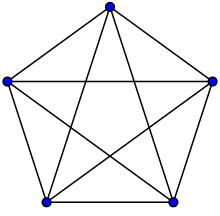
\includegraphics[width=.60\textwidth]{K5.png}
\caption{Complete graph ($K_{5}$)}
\end{minipage}
\medskip
\begin{minipage}[htbp]{.50\textwidth}
\centering
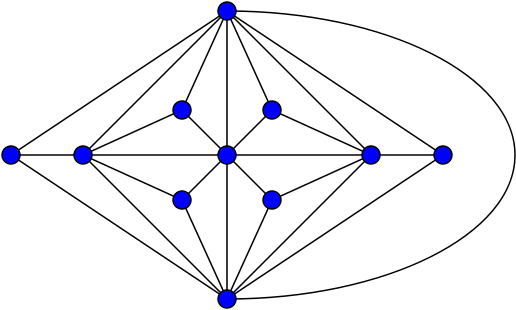
\includegraphics[width=.60\textwidth]{planare.png}
\caption{Planar graph}
\end{minipage}
\end{figure}
%1.2
\section{Matching and Perfect Matching}
Given a graph G, we want to find as many incident edges as possible.

\begin{definition}
Given a graph $G = (V,E)$, a matching $M(G)$ in $G$ is a set of pairwise non-adjacent edges; that is, no two edges share a common vertex. Or, in an equivalent form, if every vertex of G is incident to at most an edge in M, i.e. $deg(v)<= 1 \forall v\in G$.\\
This means that, in a matching M(G), all vertices can have either degree 0 or 1. In particular
\begin{itemize}
\item se deg(v) = 1, then the vertex v is matched (or saturated) if it is an endpoint of one of the edges in the matching.
\item se deg(v) = 0, then the vertex v is unmatched.
\end{itemize}
In a matching, two edges cannot be incident: if they were, then the vertex incident to these two edges would have degree 2, but this is not possible by definition.
\end{definition}

\begin{figure}[htbp]
\centering
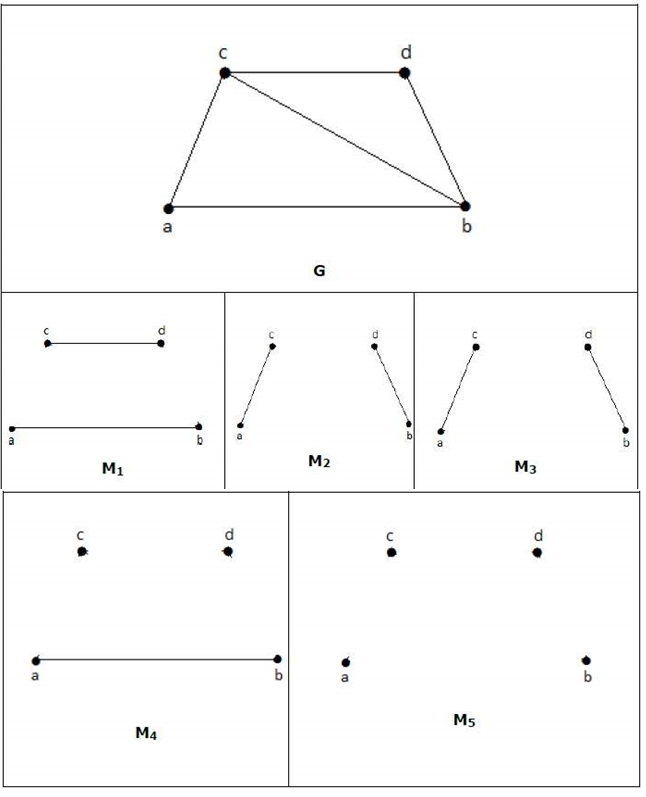
\includegraphics[width=.55\textwidth]{matching.png}
\caption{Examples of Matching of a graph G}
\end{figure}

\begin{definition}
Given $G = (V,E)$, a maximal matching is a matching M of a graph G with the property that if any edge not in M is added to M, it is no longer a matching, that is, M is maximal if it is not a subset of any other matching in graph G
\end{definition}

\begin{figure}[htbp]
\centering
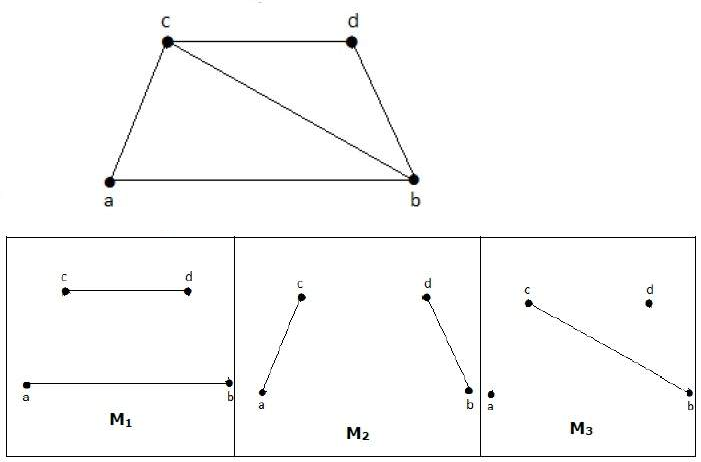
\includegraphics[width=.60\textwidth]{maximal.png}
\caption{$M_{1},M_{2},M_{3}$ are maximal matching for G}
\end{figure}

\begin{definition}
A maximum matching M(G) is a matching that contains the largest possible number of edges. There may be many maximum matchings and such number is called matching number. Note that every maximum matching is maximal, but not every maximal matching is a maximum matching. The following figure shows examples of maximum matchings in the same three graphs.
\end{definition}

\begin{figure}[htbp]
\centering
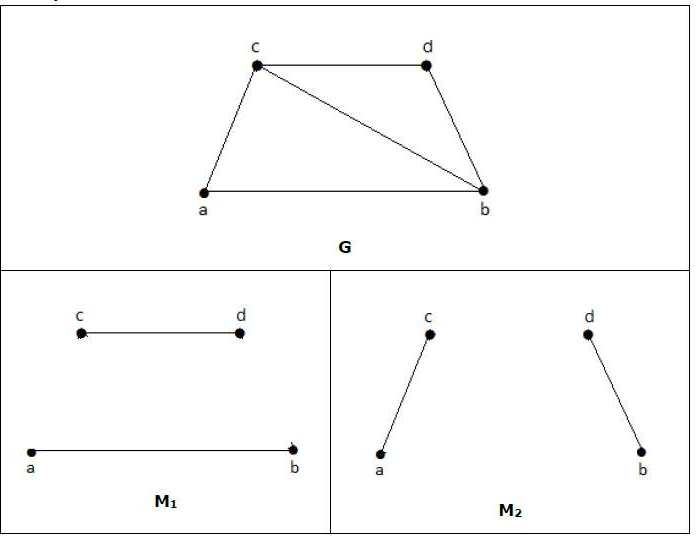
\includegraphics[width=.60\textwidth]{maximum.png}
\caption{$M_{1}$ e $M_{2}$ are maximum matching for G and the matching number is 2. Hence, using the graph G, we can form only subgraphs with at most 2 edges. For this reason we have 2 as matching number}
\end{figure}

\begin{definition}
A matching M(G) of a graph G is said to be perfect if every vertex $v \in G$ is incident to exactly one edge $e \in M$, i.e. if $deg(v) = 1 \forall v \in V$
\end{definition}

\begin{figure}[htbp]
\centering
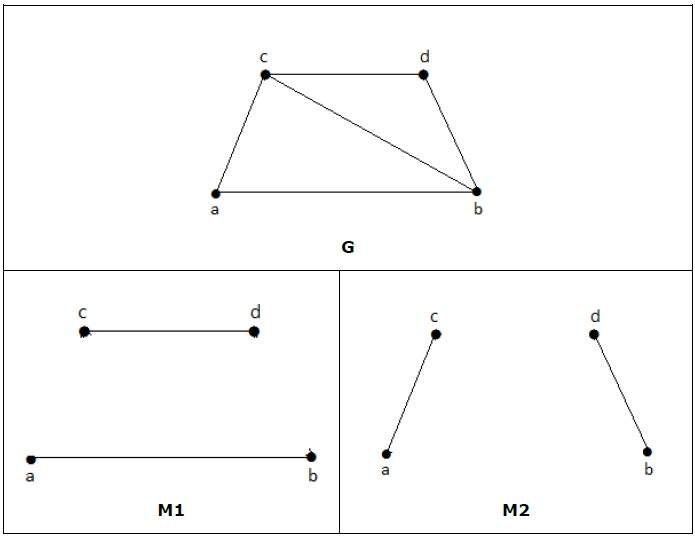
\includegraphics[width=.60\textwidth]{perfect.png}
\caption{$M_{1}$ e $M_{2}$ are examples of perfect matching for G}
\end{figure}

\begin{observation}
From the definition above, we deduce:
\begin{enumerate}
\item Every perfect matching of graph is also a maximum matching of graph, because there is no chance of adding one more edge in a perfect matching graph.. As a consequence, it is also maximal.
\item A maximum matching of graph need not be perfect.
\item If a graph G has a perfect matching, then the number of vertices |V(G)| is even. If it were odd, then the last vertex pairs with the other vertex, and finally there remains a single vertex which cannot be paired with any other vertex for which the degree is zero. It clearly violates the perfect matching principle.
\end{enumerate}
\end{observation}

\begin{figure}[htbp]
\begin{minipage}[htbp]{.80\textwidth}
\centering
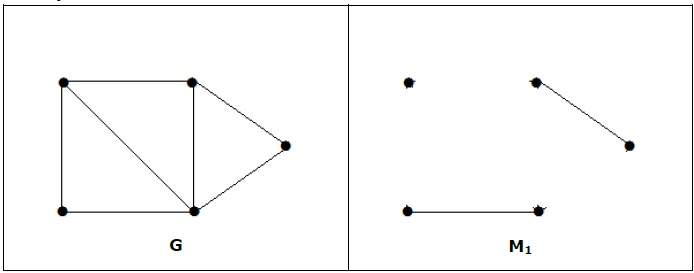
\includegraphics[width=.60\textwidth]{matching1.png}
\caption{The converse of the above statement need not be true. If G has even number of vertices, then $M_{1}$ need not be perfect.}
\end{minipage}
\begin{minipage}[htbp]{.80\textwidth}
\centering
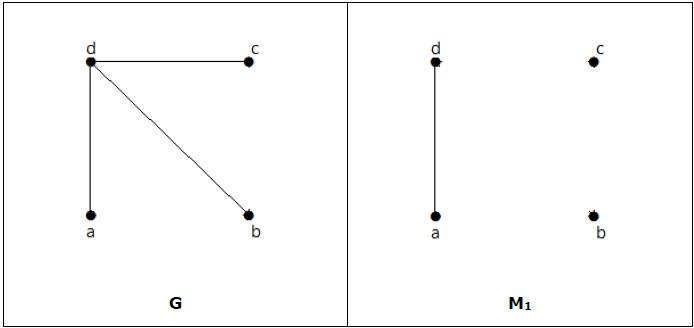
\includegraphics[width=.60\textwidth]{matching2.png}
\caption{It is matching, but it is not a perfect match, even though it has even number of vertices}
\end{minipage}
%\medskip per saltare riga
\end{figure}

%% 1.3
\section{Some examples of Perfect Matching}
To model some problems about Perfect Matching, you often use bipartite graphs. Let $G = (V,E)$ be a bipartite graph with bipartition $\left \{A,B \right \}$, i.e $V = A \cup B$ and $A \cap B = \emptyset$ and all edges link vertices from A to B. Our aim is to find a matching M in G with as many edges as possible.

\begin{definition}
A path in G which starts in A at an unmatched vertex and then contains, alternately, edges from E $\smallsetminus M$ and from M is called alternating path with respect to M.\\
An alternating path P that ends in an unmatched vertex B is called an augmenting path.
\end{definition}
To solve some problems about combinations, you use concepts about graph theory. In this section, we are going to deal with some simple examples of perfect matching and how to solve them. For this reason, we state a very useful result

\begin{theorem}[Hall, 1935]
A bipartite graph G admits a matching A if and only if
\begin{equation*}
|N(S)| \ge |S| \qquad \forall S \subseteq A
\end{equation*}
\end{theorem}
\begin{proof}
See $[1]$.
\end{proof}

\begin{example}
Suppose I have 6 gifts (labeled 1,2,3,4,5,6) to give to 5 friends (Alice, Bob, Charles, Dot, Edward). Can i distribute one gift to each person so that everyone gets something they wish? Certainly, this depends on the preferences of my friends. If none of them like any of my gifts, then I am out of luck. But even if they all like some gifts, I may still not be able to give them out satisfactiorily. For instance, if none of them like gifts 5 or 6, then I will have only 4 gifts to give to my 5 friends and so the problem admits no solutions. We exclude these two particular cases.

\begin{figure}[htbp]
\centering
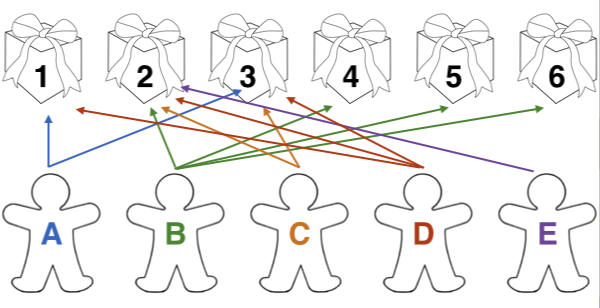
\includegraphics[width=.60\textwidth]{bambini.png}
\caption{Can every child receive the gift he/she prefers?}
\end{figure}

We can model this situation as a graph partioned into two sets: the set of the gifts and the set of the friends. By definition, it is clear that the graph is bipartite. An edge is associated to each child which denotes the preferences about the gifts (for instance, Alice wishes gift 1 or 3 and so on). Let's check if it satisfies or not Hall's theorem: we consider a subset $X = \left \{ A,C,D,E \right \}$, hence $|X| = 4$ and as a consequence $N(X) = \left \{ 1,2,3 \right \}$, so $|X| = 3$. From this, we deduce that $|X| \ge |N(X)|$, thus Hall's condition has been violated and so there no exists a matching. In other words, it is not possible to distribute to everyone the desired gift.
\end{example}

Another example is the vertex cover problem.
\begin{definition}
Let $G = (V,E)$ be a graph. A vertex cover of G is a subset $U \subseteq V$ such that every edge $e \in E$ is incident to a vertex $v \in U$.
\end{definition}
This means that every vertex in the graph is touching at least one edge. Vertex cover is a topic in graph theory that has applications in matching problems and optimization problems. A vertex cover might be a good approach to a problem where all of the edges in a graph need to be included in the solution. In particular, you ask to find minimum vertex cover. 

\begin{figure}[htbp]
\begin{minipage}[htbp]{.80\textwidth}
\centering
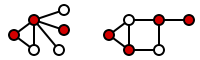
\includegraphics[width=.60\textwidth]{cover.png}
\caption{Examples of vertex cover}
\end{minipage}
\begin{minipage}[htbp]{.80\textwidth}
\centering
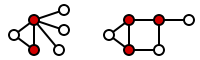
\includegraphics[width=.60\textwidth]{cover1.png}
\caption{Examples of minimum vertex cover}
\end{minipage}
%\medskip per saltare riga
\end{figure}

\begin{observation}
\begin{itemize}
We just report some properties of Vertex Cover:
\item The set of all vertices is a vertex cover;
\item Endpoints of a maximal matching form a vertex cover;
\item The complete bipartite graph $K_{m,n}$ has a minimum vertex cover given by $min\left \{m,n \right \}$.
\end{itemize}
\end{observation}

The following result establishes a link between vertex cover and perfect matching. In particular
\begin{theorem}[K\"onig, 1931]
In a bipartite graph G, the number of edges in a maximum matching is equal to the number of vertices in a minimum vertex cover.
\end{theorem}
\begin{proof}
See $[1]$.
\end{proof}

%\begin{ese}

%You have an art gallery with many hallways and turns. Your gallery is displaying very valuable paintings, and you want to keep them secure. You are planning to install security cameras in each hallway so that the cameras have every painting in view. If there is a security camera in a hallway, it can see every painting in the hallway. If there is a camera in the corner where two hallways meet (the turn), it can view paintings in both hallways. We can model this system as a graph where the nodes represent the places where the hallways cross each other or when a hallway becomes a dead end, and the edges are the hallways. Our aim is to find "strategic" places where to install security cameras.\\
%The easiest solution is to put them in every node: by definition, it is a vertex cover since all edges must be connected to at least one vertex. Doing so, we do not have any risk. However, we suppose that every security camera has a cost, so we want to find the minimum number possible of cameras in order to minimize also the costs. With this assumption, we want to solve the minimum vertex cover problem.\\
%The following picture shows some possible solutions:

\begin{figure}[htbp]
\centering
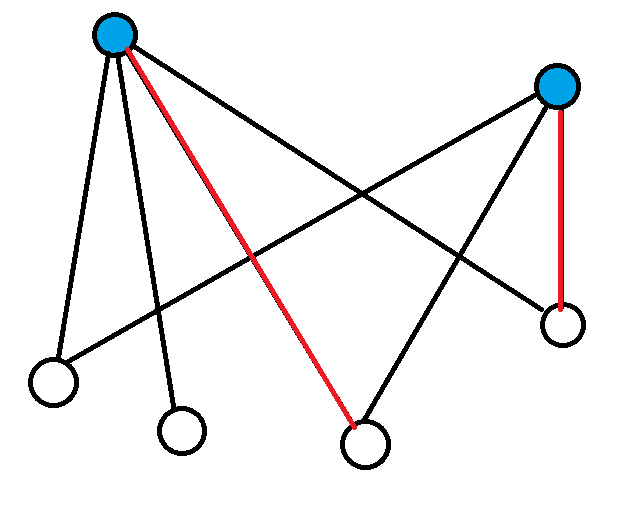
\includegraphics[width=.60\textwidth]{Pm.png}
\caption{Example of application of K\"onig Theorem: red vertices are the minimum vertex cover and blue edges are the maximum matching}
\end{figure}
%\end{ese}

